\documentclass[tikz]{standalone}

\usepackage{amsmath}
\usepackage{fontspec}

\setmainfont{TeX Gyre Termes}

\usetikzlibrary{calc}

\begin{document}

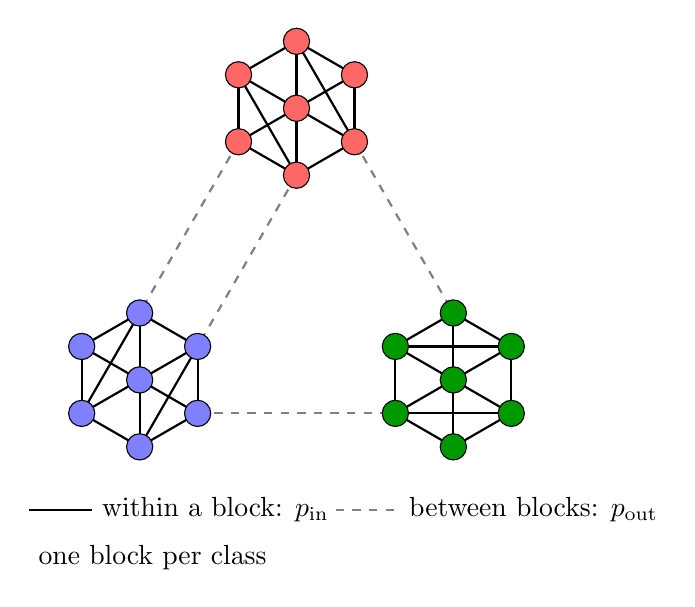
\begin{tikzpicture}[
	vertex/.style={circle, draw=black, minimum size=2.2ex, inner sep=0pt},
	intra/.style={thick},
	inter/.style={thick, dashed, gray},
]
	% Node positions: one block per class, a hexagon around a centre node
	\foreach \b/\angle in {A/90, B/210, C/330} {
		\coordinate (\b0) at (\angle:2.3);
		\foreach \i in {1, ..., 6} {
			\coordinate (\b\i) at ($ (\b0) + (\i * 60 + \angle:0.85) $);
		}
	}

	% Dense edges within each block
	\foreach \b in {A, B, C} {
		\foreach \i in {1, ..., 6} {
			\draw[intra] (\b0) -- (\b\i);
		}
		\foreach \i/\j in {1/2, 2/3, 3/4, 4/5, 5/6, 6/1, 1/3, 4/6} {
			\draw[intra] (\b\i) -- (\b\j);
		}
	}

	% Sparse edges between blocks
	\draw[inter] (A2) -- (B4);
	\draw[inter] (A3) -- (B3);
	\draw[inter] (A4) -- (C2);
	\draw[inter] (B2) -- (C4);

	% Nodes on top of the edges
	\foreach \b/\col in {A/red!60, B/blue!50, C/green!60!black} {
		\foreach \i in {0, ..., 6} {
			\node[vertex, fill=\col] at (\b\i) {};
		}
	}

	% Legend
	\begin{scope}[shift={(-3.4, -2.8)}]
		\draw[intra] (0, 0) -- (0.8, 0) node[right] {within a block: \( p_\text{in} \)};
		\draw[inter] (3.9, 0) -- (4.7, 0) node[right, black] {between blocks: \( p_\text{out} \)};
		\node[anchor=west] at (0, -0.6) {one block per class};
	\end{scope}
\end{tikzpicture}

\end{document}
